% !TeX program = xelatex
% 编译：xelatex 09-第三章引言.tex（VS Code 的 LaTeX Workshop 会读上一行，自动用 xelatex）
% 来源：2022 浙江大学《信号与系统》胡浩基老师，第三章引言及其 MATLAB 程序讲解（两段视频）。
% 体例：先讲为什么要做频率分析（已知输入输出反求冲激响应），离散情况用递推求解，连续情况引出傅里叶变换给出的 h(t)；再讲数值计算这个 h(t) 的 MATLAB 程序、结果与易错点。
% 图中曲线数据：按课上程序（及改正零值判断后的程序）用 Python 复现计算后取样，直接写成 TikZ 坐标。
\documentclass[UTF8,a4paper,11pt]{ctexart}
\usepackage{amsmath,amssymb}
\usepackage{geometry}
\geometry{margin=2.4cm}
\usepackage{xcolor}
\usepackage{mdframed}
\usepackage{booktabs}
\usepackage{needspace}
\usepackage{array}
\usepackage{enumitem}
\usepackage{tikz}
\usetikzlibrary{arrows.meta,positioning,calc,patterns}
\usepackage{float}
\usepackage{fancyhdr}
% 页眉页脚清空，只在右下角保留页号（含首页）
\fancypagestyle{plain}{%
  \fancyhf{}%
  \fancyfoot[R]{\thepage}%
  \renewcommand{\headrulewidth}{0pt}%
  \renewcommand{\footrulewidth}{0pt}}
\usepackage[hidelinks,unicode,bookmarksnumbered,bookmarksopen=true,bookmarksopenlevel=2,pdftitle={第三章引言}]{hyperref}
\usepackage{bookmark}% XeTeX 下 hyperref 自带的大纲不生效，用 bookmark 宏包生成 PDF 书签（需编译两遍）

\setCJKmainfont{Songti SC}[BoldFont={Songti SC Bold}]
\setCJKsansfont{PingFang SC}
\setCJKmonofont{PingFang SC}

\newmdenv[backgroundcolor=blue!4,linecolor=blue!50!black,linewidth=1pt,innertopmargin=6pt,innerbottommargin=6pt]{rememberbox}
\newenvironment{remember}{\begin{rememberbox}\textbf{重点}\par\smallskip}{\end{rememberbox}}
\newmdenv[backgroundcolor=yellow!8,linecolor=orange!70!black,linewidth=1pt,innertopmargin=6pt,innerbottommargin=6pt]{notebox}
\newenvironment{note}{\begin{notebox}\textbf{说明}\par\smallskip}{\end{notebox}}
% 代码框：灰底，内放 verbatim
\newmdenv[backgroundcolor=gray!6,linecolor=gray!60,linewidth=0.6pt,innertopmargin=4pt,innerbottommargin=4pt,innerleftmargin=8pt]{codebox}

% ---------------------------------------------------------------- 画图用的小宏
% 坐标轴：\taxes[自变量名]{横轴起点}{横轴终点}{纵轴顶端}{纵轴底端}。原点标 0（放在左下，避开纵轴）。
\newcommand{\taxes}[5][t]{%
  \draw[->] (#2,0) -- (#3,0) node[right,font=\scriptsize] {$#1$};
  \draw[->] (0,#5) -- (0,#4);
  \node[anchor=north east,font=\tiny,gray!60!black,inner sep=1pt] at (0,-0.02) {$0$};}
% 横轴刻度 \xt{位置}{标签}（标在轴下方）、\xtu{位置}{标签}（标在轴上方）、纵轴刻度 \yt{位置}{标签}：刻度线 + 白底数字。
\newcommand{\xt}[2]{\draw (#1,0) -- (#1,-0.1) node[anchor=north,font=\tiny,gray!60!black,fill=white,inner sep=0.6pt] {$#2$};}
\newcommand{\xtu}[2]{\draw (#1,0) -- (#1,0.1) node[anchor=south,font=\tiny,gray!60!black,fill=white,inner sep=0.6pt] {$#2$};}
\newcommand{\yt}[2]{\draw (0,#1) -- (-0.1,#1) node[anchor=east,font=\tiny,gray!60!black,fill=white,inner sep=0.6pt] {$#2$};}
% 火柴杆：\stem{n}{值}{颜色}，值标在杆顶
\newcommand{\stem}[3]{\draw[thick,#3] (#1,0) -- (#1,#2); \fill[#3] (#1,#2) circle (1.6pt);
  \node[anchor=south,font=\tiny,#3,inner sep=1.5pt] at (#1,#2) {$#2$};}
\newcommand{\opsym}[3]{\node[font=\Large] at (#1,#2) {#3};}
\tikzset{>=stealth,
  sig/.style={thick,blue!60!black},
  res/.style={thick,red!70!black},
  outc/.style={thick,green!45!black}}

% ---------------------------------------------------------------- 标题层级
\definecolor{secblue}{RGB}{31,78,121}
\definecolor{exorange}{RGB}{190,90,10}
\definecolor{ptteal}{RGB}{0,110,110}
\ctexset{
  section={format=\raggedright\Large\bfseries\color{secblue},
           beforeskip=3.2ex plus 1ex minus .5ex, afterskip=1.4ex,
           aftertitle={\par\nobreak\vspace{-1.1ex}\noindent\textcolor{secblue}{\rule{\linewidth}{0.8pt}}\par\nobreak\vspace{0.6ex}}},
  subsection={format=\raggedright\large\bfseries\color{secblue},
              beforeskip=2.4ex plus .8ex minus .4ex, afterskip=1.0ex}
}
% 例题标题：\example{标题}{结论}{附注}，附注一般留空。
\newcounter{ex}[section]
\newcommand{\example}[3]{%
  \refstepcounter{ex}\phantomsection
  \addcontentsline{toc}{subsubsection}{例 \theex\ #1（#2）}%
  \par\addvspace{1.6ex}\noindent
  {\setlength{\fboxsep}{3pt}%
   \colorbox{exorange}{\textcolor{white}{\textbf{例~\theex}}}\ %
   \textcolor{exorange}{\textbf{#1}}\ {\footnotesize\textcolor{gray!70!black}{#3}}%
   \hfill\colorbox{exorange!12}{\small\textcolor{exorange}{#2}}\par}%
  \nobreak\vskip0.6ex\relax\csname @afterheading\endcsname}
% 小标题（接着同一段往下写，不进大纲）：青色三角 + 粗体。
\newcommand{\point}[1]{\par\addvspace{1ex}\noindent\textcolor{ptteal}{$\blacktriangleright$\,\textbf{#1}}\ }

\title{第三章引言：为什么要做频率分析\\\large 浙江大学 2022《信号与系统》（胡浩基）第三章听课笔记}
\author{}
\date{}

\begin{document}
\pagestyle{plain}
\maketitle

%==================================================================
\section{为什么要做频率分析}\label{sec:why}
第三章的章名是「连续时间信号与系统的频率分析(frequency analysis)」，核心是傅里叶变换(Fourier transform)。傅里叶(Fourier)是法国科学家。

\point{第二章留下的问题。}第二章解决了「已知 $x(t)$、$h(t)$，求 $y(t)$」：LTI 系统的输出是输入与冲激响应的卷积，
\[
y(t)=x(t)\ast h(t).
\]
但它没有回答反过来的问题：\textbf{已知 $x(t)$ 和 $y(t)$，怎样求 $h(t)$？}这相当于解方程。好比学了 $2\times3=6$ 之后，还要会回答「$2$ 乘以几等于 $6$」。

\begin{remember}
\begin{itemize}[nosep]
\item 正问题：已知 $x$、$h$，求 $y=x\ast h$（第二章）。
\item 反问题：已知 $x$、$y$，求满足 $x\ast h=y$ 的 $h$。离散、有限长时可以递推求解（第 \ref{sec:disc} 节）；连续时用第二章的知识做不到，要靠第三章的傅里叶变换（第 \ref{sec:cont} 节）。
\end{itemize}
\end{remember}

%==================================================================
\section{离散情况：递推求 \texorpdfstring{$h[n]$}{h[n]}}\label{sec:disc}

\example{已知 \texorpdfstring{$x[n]$、$y[n]$ 求 $h[n]$}{x[n]、y[n] 求 h[n]}}{$h[n]=[2,4,4]$}{}
\textbf{题目}：$x[n]=[1,2,1]$，$y[n]=[2,8,14,12,4]$（都从 $n=0$ 开始），$x[n]\ast h[n]=y[n]$，求 $h[n]$。

\point{第一步：$h[n]$ 有几个数。}长度为 $N_1$ 与 $N_2$ 的两个序列卷积，结果长度为 $N_1+N_2-1$（第 04 篇）。这里 $N_1=3$，$y$ 的长度为 $5$：
\[
3+N_2-1=5\ \Longrightarrow\ N_2=3 .
\]
\point{第二步：用交换律，翻转 $x$ 而不翻转 $h$。}把 $h[n]$ 的三个未知数正着写，把 $x[n]$ 翻转成 $x[-n]$（$1,2,1$ 翻转后仍是 $1,2,1$），从左往右逐格滑动，每滑一格对应 $y$ 的一个数，每次只多出一个未知数：

\begin{center}
\renewcommand{\arraystretch}{1.3}
\begin{tabular}{cccl}
\toprule
$y$ 的第几个数 & 重叠的乘积之和 & $=y[n]$ & 解出\\
\midrule
$y[0]$ & $1\cdot h[0]$ & $2$ & $h[0]=2$\\
$y[1]$ & $2\cdot h[0]+1\cdot h[1]=4+h[1]$ & $8$ & $h[1]=4$\\
$y[2]$ & $1\cdot h[0]+2\cdot h[1]+1\cdot h[2]=2+8+h[2]$ & $14$ & $h[2]=4$\\
\bottomrule
\end{tabular}
\end{center}

\point{第三步：用剩下的数验算。}
\[
y[3]=1\cdot h[1]+2\cdot h[2]=4+8=12,\qquad y[4]=1\cdot h[2]=4,
\]
与已知的 $y$ 一致，所以 $h[n]=[2,4,4]$。

\begin{figure}[H]
\centering
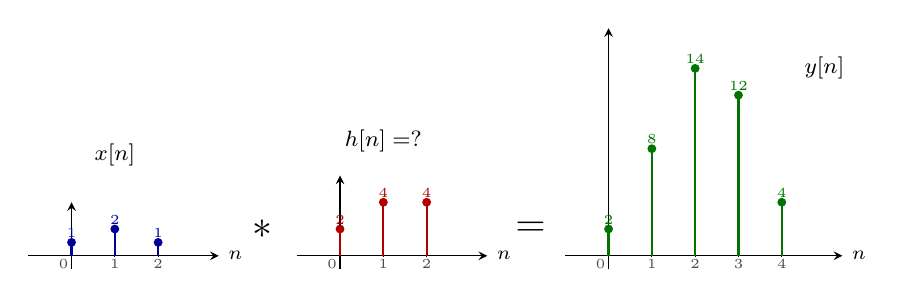
\begin{tikzpicture}[x=0.55cm,y=0.17cm]
  \begin{scope}
    \taxes[n]{-1}{3.4}{4}{-1}
    \stem{0}{1}{blue!60!black}\stem{1}{2}{blue!60!black}\stem{2}{1}{blue!60!black}
    \xt{1}{1}\xt{2}{2}
    \node[font=\footnotesize,anchor=south] at (1,6) {$x[n]$};
  \end{scope}
  \opsym{4.4}{2}{$\ast$}
  \begin{scope}[shift={(6.2,0)}]
    \taxes[n]{-1}{3.4}{6}{-1}
    \stem{0}{2}{red!70!black}\stem{1}{4}{red!70!black}\stem{2}{4}{red!70!black}
    \xt{1}{1}\xt{2}{2}
    \node[font=\footnotesize,anchor=south] at (1,7) {$h[n]=?$};
  \end{scope}
  \opsym{10.6}{2}{$=$}
  \begin{scope}[shift={(12.4,0)}]
    \taxes[n]{-1}{5.4}{17}{-1}
    \stem{0}{2}{green!45!black}\stem{1}{8}{green!45!black}\stem{2}{14}{green!45!black}\stem{3}{12}{green!45!black}\stem{4}{4}{green!45!black}
    \xt{1}{1}\xt{2}{2}\xt{3}{3}\xt{4}{4}
    \node[font=\footnotesize,anchor=west] at (4.3,14) {$y[n]$};
  \end{scope}
\end{tikzpicture}
\caption{$[1,2,1]\ast h[n]=[2,8,14,12,4]$，递推解出 $h[n]=[2,4,4]$（红色）。}
\end{figure}

\begin{remember}
\textbf{一般的递推}（要求 $x[0]\ne0$，序列都从 $n=0$ 开始）：由 $y[n]=\sum_{k=0}^{n}x[k]\,h[n-k]$，
\[
h[0]=\frac{y[0]}{x[0]},\qquad
h[n]=\frac{1}{x[0]}\Big(y[n]-\sum_{k=1}^{n}x[k]\,h[n-k]\Big),\quad n=1,2,\dots,N_2-1 .
\]
离散、有限长时，求 $h[n]$ 只是递推运算；剩下的 $y$ 值用来验算。
\end{remember}

\point{MATLAB 作业一。}给定 $x[n]$ 和 $y[n]$，编程求出 $h[n]$。

%==================================================================
\section{连续情况：第二章的方法做不到}\label{sec:cont}

\example{方波卷积得三角波，反求 \texorpdfstring{$h(t)$}{h(t)}}{要用傅里叶变换}{}
\textbf{题目}：$x(t)$ 是 $[0,2]$ 上高为 $1$ 的方波，$y(t)$ 是 $[0,2]$ 上的等腰三角形（$t=1$ 处高为 $1$），$x(t)\ast h(t)=y(t)$，求 $h(t)$。

\begin{figure}[H]
\centering
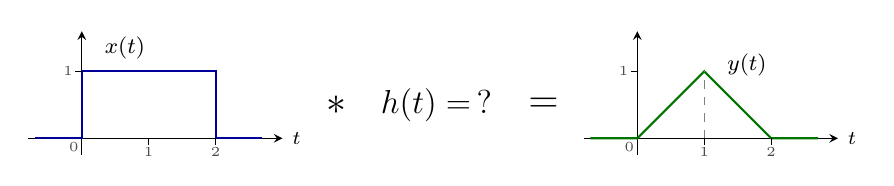
\begin{tikzpicture}[x=0.85cm,y=0.85cm]
  \begin{scope}
    \taxes{-0.8}{3.0}{1.6}{-0.25}
    \draw[sig] (-0.7,0) -- (0,0) -- (0,1) -- (2,1) -- (2,0) -- (2.7,0);
    \xt{1}{1}\xt{2}{2}\yt{1}{1}
    \node[font=\footnotesize,anchor=west] at (0.2,1.35) {$x(t)$};
  \end{scope}
  \opsym{3.8}{0.5}{$\ast$}
  \node[font=\large] at (5.3,0.5) {$h(t)=\,?$};
  \opsym{6.9}{0.5}{$=$}
  \begin{scope}[shift={(8.3,0)}]
    \taxes{-0.8}{3.0}{1.6}{-0.25}
    \draw[outc] (-0.7,0) -- (0,0) -- (1,1) -- (2,0) -- (2.7,0);
    \draw[dashed,gray] (1,0) -- (1,1);
    \xt{1}{1}\xt{2}{2}\yt{1}{1}
    \node[font=\footnotesize,anchor=west] at (1.2,1.1) {$y(t)$};
  \end{scope}
\end{tikzpicture}
\caption{已知方波输入与三角波输出，求冲激响应 $h(t)$。}
\end{figure}

用第二章的知识解不出来。
\begin{remember}
学了第三章傅里叶变换的卷积性质，可以得到
\[
h(t)=\frac1\pi\int_{-\infty}^{+\infty}\frac{\sin^2\!\big(\frac{\omega}{2}\big)}{\omega\,\sin\omega}\,\cos(\omega t)\,\mathrm{d}\omega .
\]
\end{remember}

这个表达式有三处「奇怪」：
\begin{enumerate}[nosep]
\item \textbf{它确实是 $t$ 的函数。}被积函数里有 $\omega$ 和 $t$ 两个变量，对 $\omega$ 积分后 $\omega$ 被积掉，只剩 $t$。
\item \textbf{它与取值范围规则矛盾。}按「$y$ 的最左端 $=$ $x$ 的最左端 $+$ $h$ 的最左端」，$x$、$y$ 都从 $0$ 开始，$h$ 应从 $0$ 开始；按最右端，$x$、$y$ 都到 $2$ 结束，$h$ 应在 $0$ 结束。但这个 $h(t)$ 在 $(-\infty,+\infty)$ 上都有值。原因是：卷积时 $h$ 左右两边的值会相互抵消，而抵消的前提是积分严格地从 $-\infty$ 积到 $+\infty$。用数值方法计算时必须截断，得到的 $y$ 只能是近似值。
\item \textbf{为什么会和 $\cos(\omega t)$ 联系在一起？}这要学完第三章傅里叶变换才能回答。
\end{enumerate}

\point{MATLAB 作业二。}
\begin{enumerate}[nosep]
\item 编程求 $h(t)$ 在 $t\in[-10,10]$ 上的近似图像（积分截断到有限范围）；
\item 将得到的 $h(t)$ 与 $x(t)$ 卷积，看 $y(t)$ 的样子是否接近三角波。
\end{enumerate}

%==================================================================
\section{数值计算 \texorpdfstring{$h(t)$}{h(t)} 的 MATLAB 程序}\label{sec:matlab}

\subsection{编程前先化简}
先分析表达式，把计算量降到最小。

\point{被积函数是 $\omega$ 的偶函数，积分只算正半轴。}$\sin\frac{\omega}{2}$ 是奇函数，平方后是偶函数；分母 $\omega$ 与 $\sin\omega$ 都是奇函数，乘积是偶函数；$\cos(\omega t)$ 也是 $\omega$ 的偶函数。偶函数除以、乘以偶函数仍是偶函数，所以
\[
h(t)=\frac2\pi\int_{0}^{+\infty}\frac{\sin^2\!\big(\frac{\omega}{2}\big)}{\omega\,\sin\omega}\,\cos(\omega t)\,\mathrm{d}\omega .
\]
\point{$h(t)$ 是 $t$ 的偶函数，只算 $t\ge0$。}$t$ 只出现在 $\cos(\omega t)$ 里，$\cos$ 是偶函数，所以 $h(-t)=h(t)$。算出正半轴后，翻转得到负半轴。

\point{积分上限截断到 $\omega_0$。}计算机只能处理有限，必须在某个 $\omega_0>0$ 处截断：
\[
h(t)\approx\frac2\pi\int_{0}^{\omega_0}\frac{\sin^2\!\big(\frac{\omega}{2}\big)}{\omega\,\sin\omega}\,\cos(\omega t)\,\mathrm{d}\omega ,\qquad \omega_0=20 .
\]
截断会带来误差，表现为结果上的起伏。

\point{积分用小矩形求和近似。}把 $\omega$ 轴按步长 $\Delta\omega$（程序里的 \texttt{intervalW}，取 $0.001$）切成小段，每段面积近似为「函数值 $\times\,\Delta\omega$」，全部加起来。步长可以按电脑的计算能力调大或调小。

\begin{figure}[H]
\centering
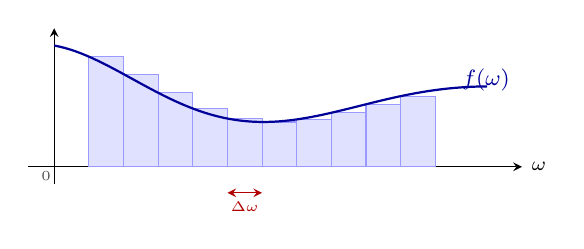
\begin{tikzpicture}[x=1.1cm,y=1.1cm]
  \taxes[\omega]{-0.3}{5.4}{1.6}{-0.2}
  \foreach \a in {0.4,0.8,...,4.4}{
    \pgfmathsetmacro{\v}{0.5+0.6*exp(-0.3*\a)*cos(1.2*\a r)+0.3}
    \fill[blue!12] (\a,0) rectangle ({\a+0.4},\v);
    \draw[blue!40] (\a,0) rectangle ({\a+0.4},\v);}
  \draw[sig,domain=0:5,samples=80] plot (\x,{0.5+0.6*exp(-0.3*\x)*cos(1.2*\x r)+0.3});
  \draw[<->,red!70!black] (2.0,-0.3) -- (2.4,-0.3) node[midway,below,font=\tiny] {$\Delta\omega$};
  \node[font=\footnotesize,blue!60!black,anchor=west] at (4.6,1.0) {$f(\omega)$};
\end{tikzpicture}
\caption{数值积分：每个小矩形的面积是 $f(\omega)\,\Delta\omega$，全部相加近似积分。$\Delta\omega$ 越小越准，计算量越大。}
\end{figure}

\subsection{程序}
\begin{codebox}
\small
\begin{verbatim}
T0 = 50;
intervalT = 0.001;
t = 0:intervalT:T0;

W0 = 20;
intervalW = 0.001;
w = 0:intervalW:W0;
functionW = zeros(1, length(w));
for i = 1:length(w)
    if sin(w(i))>1e-6    % 零值判断（应写 abs(sin(w(i)))>1e-6，见 4.4 节）
        functionW(i) = sin(0.5*w(i))^2/(w(i).*sin(w(i)));
    else
        functionW(i) = 0.25;   % 趋于 0 的点取极限 0.25
    end
end

% 这里是求 h
h = zeros(1, length(t));
for i = 1:length(t)
    for j = 1:length(functionW)
        h(i) = h(i)+functionW(j)*cos(w(j)*t(i))*intervalW;
    end
end
h = 2*h/pi;

% 由于 h(t) 是偶函数，因此将图像翻转到负半轴。
t = [-t(end:-1:2), t];
h = [h(end:-1:2), h];

% 画 h(t)。
subplot(2,1,1);
plot(t, h);

% 这里是验证求出的 h(t) 和 x(t) 卷积后获得的 y(t) 是什么样子。
newT = -10:intervalT:10;
y = zeros(1, length(newT));
for i = 1:length(newT)
    time = newT(i);
    for tao = -20:0.001:20
        hindex = 1+round((tao-t(1))/intervalT);
        if time-tao>0 && time-tao<2 && hindex>=1 && hindex<=length(h)
            y(i) = y(i)+h(hindex)*0.001;
        end
    end
end
\end{verbatim}
\end{codebox}
（最后画 $y(t)$ 的两行与画 $h(t)$ 相同，用 \texttt{subplot(2,1,2)}。）

\subsection{程序要点}
\point{分母为 $0$ 要特殊处理。}$\omega=0$ 时分母 $\omega\sin\omega=0$。编程语言一般不会替你检查分母是否为 $0$，必须自己判断：分母不为 $0$ 时照公式算；为 $0$ 时取极限。$\omega\to0$ 时 $\sin\frac\omega2\approx\frac\omega2$、$\sin\omega\approx\omega$，所以
\[
\lim_{\omega\to0}\frac{\sin^2\!\big(\frac{\omega}{2}\big)}{\omega\,\sin\omega}=\lim_{\omega\to0}\frac{\omega^2/4}{\omega^2}=\frac14 ,
\]
程序里写 \texttt{0.25}。判断「是否为 $0$」用 $10^{-6}$（\texttt{1e-6}）作阈值，而不是直接与 $0$ 比较。

\point{求 $h$ 就是两重循环。}外层对每个 $t$，内层对每个 $\omega$ 累加「函数值 $\times\cos(\omega t)\times\Delta\omega$」；常数 $\frac2\pi$ 留到最后统一乘。

\point{翻转与拼接。}
\begin{itemize}[nosep]
\item \texttt{t(end)} 取数组最后一个元素；\texttt{end:-1:2} 表示下标从最后一个每次减 $1$ 到第 $2$ 个，即倒序（不含第 $1$ 个，避免 $t=0$ 重复一次）。例如 \texttt{x=[1 2 3 4]}，\texttt{x(end:-1:1)} 得 \texttt{[4 3 2 1]}。
\item \texttt{[x, y]} 把两个行向量拼成一个，例如 \texttt{[1 2 3 4]} 与 \texttt{[5 6 7 8]} 拼成 \texttt{[1 2 3 4 5 6 7 8]}。
\item 所以 \texttt{t=[-t(end:-1:2), t]} 把 $t$ 扩到负半轴；$h$ 是偶函数，负半轴的值就是正半轴倒过来，\texttt{h=[h(end:-1:2), h]}。
\end{itemize}
MATLAB 可以在命令行里随手做实验，选中几行代码复制到命令窗口运行就能看结果。这些数组操作与 Python 的写法基本一一对应。

\point{求 $y$ 用交换律后的卷积公式。}
\[
y(t)=\int_{-\infty}^{+\infty}h(\tau)\,x(t-\tau)\,\mathrm{d}\tau .
\]
$x(t-\tau)$ 只在 $0<t-\tau<2$ 时为 $1$，所以程序只在满足下面条件时累加 \texttt{h(hindex)*0.001}：
\begin{center}\small\texttt{time-tao>0 \&\& time-tao<2}\end{center}
下标由
\begin{center}\small\texttt{hindex = 1+round((tao-t(1))/intervalT)}\end{center}
算出，它把 $\tau$ 换算成 $h$ 数组的下标（\texttt{t(1)} 是 $-50$）；条件里另外两项 \texttt{hindex>=1}、\texttt{hindex<=length(h)} 保证下标不越界。

\subsection{运行结果与近似}
\begin{figure}[H]
\centering
\begin{tikzpicture}
  \begin{scope}[x=0.62cm,y=0.42cm]
    \draw[->] (-10.4,0) -- (10.6,0) node[right,font=\scriptsize] {$t$};
    \draw[->] (0,-2.9) -- (0,5.0);
    \draw[blue!60!black,line width=0.35pt] plot coordinates {(-10.00,1.663) (-9.98,1.583) (-9.96,1.472) (-9.94,1.337) (-9.92,1.185) (-9.90,1.024) (-9.88,0.863) (-9.86,0.709) (-9.84,0.568) (-9.82,0.445) (-9.80,0.343) (-9.78,0.263) (-9.76,0.203) (-9.74,0.162) (-9.72,0.135) (-9.70,0.117) (-9.68,0.104) (-9.66,0.091) (-9.64,0.074) (-9.62,0.049) (-9.60,0.016) (-9.58,-0.027) (-9.56,-0.079) (-9.54,-0.138) (-9.52,-0.200) (-9.50,-0.264) (-9.48,-0.325) (-9.46,-0.381) (-9.44,-0.429) (-9.42,-0.468) (-9.40,-0.497) (-9.38,-0.519) (-9.36,-0.534) (-9.34,-0.547) (-9.32,-0.561) (-9.30,-0.581) (-9.28,-0.610) (-9.26,-0.653) (-9.24,-0.711) (-9.22,-0.787) (-9.20,-0.880) (-9.18,-0.987) (-9.16,-1.106) (-9.14,-1.231) (-9.12,-1.355) (-9.10,-1.471) (-9.08,-1.572) (-9.06,-1.650) (-9.04,-1.700) (-9.02,-1.717) (-9.00,-1.698) (-8.98,-1.644) (-8.96,-1.555) (-8.94,-1.437) (-8.92,-1.295) (-8.90,-1.137) (-8.88,-0.971) (-8.86,-0.806) (-8.84,-0.649) (-8.82,-0.508) (-8.80,-0.388) (-8.78,-0.290) (-8.76,-0.217) (-8.74,-0.166) (-8.72,-0.134) (-8.70,-0.116) (-8.68,-0.107) (-8.66,-0.100) (-8.64,-0.089) (-8.62,-0.071) (-8.60,-0.041) (-8.58,0.001) (-8.56,0.056) (-8.54,0.121) (-8.52,0.192) (-8.50,0.265) (-8.48,0.336) (-8.46,0.400) (-8.44,0.453) (-8.42,0.494) (-8.40,0.523) (-8.38,0.540) (-8.36,0.549) (-8.34,0.555) (-8.32,0.563) (-8.30,0.579) (-8.28,0.609) (-8.26,0.657) (-8.24,0.725) (-8.22,0.816) (-8.20,0.926) (-8.18,1.053) (-8.16,1.190) (-8.14,1.330) (-8.12,1.464) (-8.10,1.585) (-8.08,1.682) (-8.06,1.750) (-8.04,1.783) (-8.02,1.777) (-8.00,1.733) (-7.98,1.652) (-7.96,1.539) (-7.94,1.400) (-7.92,1.243) (-7.90,1.076) (-7.88,0.908) (-7.86,0.748) (-7.84,0.601) (-7.82,0.472) (-7.80,0.366) (-7.78,0.282) (-7.76,0.220) (-7.74,0.177) (-7.72,0.149) (-7.70,0.130) (-7.68,0.117) (-7.66,0.104) (-7.64,0.086) (-7.62,0.061) (-7.60,0.026) (-7.58,-0.018) (-7.56,-0.072) (-7.54,-0.132) (-7.52,-0.197) (-7.50,-0.263) (-7.48,-0.326) (-7.46,-0.384) (-7.44,-0.434) (-7.42,-0.475) (-7.40,-0.506) (-7.38,-0.529) (-7.36,-0.546) (-7.34,-0.559) (-7.32,-0.574) (-7.30,-0.594) (-7.28,-0.623) (-7.26,-0.666) (-7.24,-0.725) (-7.22,-0.802) (-7.20,-0.896) (-7.18,-1.005) (-7.16,-1.127) (-7.14,-1.256) (-7.12,-1.385) (-7.10,-1.508) (-7.08,-1.616) (-7.06,-1.703) (-7.04,-1.761) (-7.02,-1.786) (-7.00,-1.774) (-6.98,-1.726) (-6.96,-1.641) (-6.94,-1.524) (-6.92,-1.382) (-6.90,-1.220) (-6.88,-1.048) (-6.86,-0.875) (-6.84,-0.709) (-6.82,-0.558) (-6.80,-0.427) (-6.78,-0.320) (-6.76,-0.239) (-6.74,-0.182) (-6.72,-0.146) (-6.70,-0.126) (-6.68,-0.116) (-6.66,-0.110) (-6.64,-0.102) (-6.62,-0.085) (-6.60,-0.057) (-6.58,-0.016) (-6.56,0.040) (-6.54,0.106) (-6.52,0.181) (-6.50,0.259) (-6.48,0.336) (-6.46,0.406) (-6.44,0.465) (-6.42,0.510) (-6.40,0.542) (-6.38,0.560) (-6.36,0.570) (-6.34,0.574) (-6.32,0.581) (-6.30,0.595) (-6.28,0.623) (-6.26,0.671) (-6.24,0.741) (-6.22,0.834) (-6.20,0.950) (-6.18,1.084) (-6.16,1.231) (-6.14,1.381) (-6.12,1.526) (-6.10,1.656) (-6.08,1.762) (-6.06,1.836) (-6.04,1.872) (-6.02,1.868) (-6.00,1.823) (-5.98,1.739) (-5.96,1.620) (-5.94,1.475) (-5.92,1.311) (-5.90,1.137) (-5.88,0.962) (-5.86,0.795) (-5.84,0.643) (-5.82,0.510) (-5.80,0.400) (-5.78,0.312) (-5.76,0.247) (-5.74,0.201) (-5.72,0.170) (-5.70,0.149) (-5.68,0.133) (-5.66,0.117) (-5.64,0.097) (-5.62,0.070) (-5.60,0.034) (-5.58,-0.011) (-5.56,-0.065) (-5.54,-0.126) (-5.52,-0.191) (-5.50,-0.257) (-5.48,-0.322) (-5.46,-0.382) (-5.44,-0.435) (-5.42,-0.479) (-5.40,-0.514) (-5.38,-0.541) (-5.36,-0.562) (-5.34,-0.579) (-5.32,-0.596) (-5.30,-0.617) (-5.28,-0.647) (-5.26,-0.688) (-5.24,-0.745) (-5.22,-0.819) (-5.20,-0.910) (-5.18,-1.019) (-5.16,-1.142) (-5.14,-1.275) (-5.12,-1.411) (-5.10,-1.543) (-5.08,-1.664) (-5.06,-1.765) (-5.04,-1.839) (-5.02,-1.879) (-5.00,-1.882) (-4.98,-1.845) (-4.96,-1.768) (-4.94,-1.655) (-4.92,-1.510) (-4.90,-1.343) (-4.88,-1.161) (-4.86,-0.975) (-4.84,-0.794) (-4.82,-0.627) (-4.80,-0.481) (-4.78,-0.360) (-4.76,-0.268) (-4.74,-0.203) (-4.72,-0.163) (-4.70,-0.142) (-4.68,-0.133) (-4.66,-0.130) (-4.64,-0.124) (-4.62,-0.110) (-4.60,-0.083) (-4.58,-0.041) (-4.56,0.018) (-4.54,0.089) (-4.52,0.171) (-4.50,0.257) (-4.48,0.341) (-4.46,0.418) (-4.44,0.483) (-4.42,0.533) (-4.40,0.566) (-4.38,0.586) (-4.36,0.594) (-4.34,0.596) (-4.32,0.600) (-4.30,0.612) (-4.28,0.640) (-4.26,0.690) (-4.24,0.764) (-4.22,0.864) (-4.20,0.989) (-4.18,1.135) (-4.16,1.293) (-4.14,1.457) (-4.12,1.614) (-4.10,1.755) (-4.08,1.870) (-4.06,1.952) (-4.04,1.993) (-4.02,1.990) (-4.00,1.944) (-3.98,1.856) (-3.96,1.733) (-3.94,1.581) (-3.92,1.409) (-3.90,1.227) (-3.88,1.044) (-3.86,0.869) (-3.84,0.708) (-3.82,0.567) (-3.80,0.449) (-3.78,0.355) (-3.76,0.283) (-3.74,0.231) (-3.72,0.194) (-3.70,0.169) (-3.68,0.150) (-3.66,0.131) (-3.64,0.110) (-3.62,0.083) (-3.60,0.048) (-3.58,0.004) (-3.56,-0.049) (-3.54,-0.109) (-3.52,-0.175) (-3.50,-0.243) (-3.48,-0.311) (-3.46,-0.376) (-3.44,-0.435) (-3.42,-0.487) (-3.40,-0.530) (-3.38,-0.564) (-3.36,-0.591) (-3.34,-0.612) (-3.32,-0.630) (-3.30,-0.650) (-3.28,-0.676) (-3.26,-0.711) (-3.24,-0.761) (-3.22,-0.827) (-3.20,-0.913) (-3.18,-1.018) (-3.16,-1.142) (-3.14,-1.280) (-3.12,-1.426) (-3.10,-1.575) (-3.08,-1.717) (-3.06,-1.844) (-3.04,-1.946) (-3.02,-2.015) (-3.00,-2.045) (-2.98,-2.032) (-2.96,-1.974) (-2.94,-1.872) (-2.92,-1.732) (-2.90,-1.560) (-2.88,-1.366) (-2.86,-1.162) (-2.84,-0.957) (-2.82,-0.763) (-2.80,-0.589) (-2.78,-0.443) (-2.76,-0.327) (-2.74,-0.244) (-2.72,-0.191) (-2.70,-0.163) (-2.68,-0.152) (-2.66,-0.150) (-2.64,-0.150) (-2.62,-0.141) (-2.60,-0.119) (-2.58,-0.080) (-2.56,-0.022) (-2.54,0.054) (-2.52,0.143) (-2.50,0.240) (-2.48,0.337) (-2.46,0.428) (-2.44,0.506) (-2.42,0.567) (-2.40,0.610) (-2.38,0.634) (-2.36,0.643) (-2.34,0.644) (-2.32,0.644) (-2.30,0.652) (-2.28,0.676) (-2.26,0.724) (-2.24,0.800) (-2.22,0.908) (-2.20,1.045) (-2.18,1.208) (-2.16,1.388) (-2.14,1.575) (-2.12,1.756) (-2.10,1.921) (-2.08,2.057) (-2.06,2.154) (-2.04,2.204) (-2.02,2.206) (-2.00,2.157) (-1.98,2.061) (-1.96,1.925) (-1.94,1.758) (-1.92,1.569) (-1.90,1.370) (-1.88,1.172) (-1.86,0.982) (-1.84,0.810) (-1.82,0.660) (-1.80,0.534) (-1.78,0.433) (-1.76,0.354) (-1.74,0.295) (-1.72,0.251) (-1.70,0.217) (-1.68,0.189) (-1.66,0.163) (-1.64,0.135) (-1.62,0.103) (-1.60,0.065) (-1.58,0.022) (-1.56,-0.028) (-1.54,-0.083) (-1.52,-0.143) (-1.50,-0.206) (-1.48,-0.272) (-1.46,-0.339) (-1.44,-0.405) (-1.42,-0.469) (-1.40,-0.528) (-1.38,-0.582) (-1.36,-0.628) (-1.34,-0.666) (-1.32,-0.696) (-1.30,-0.718) (-1.28,-0.734) (-1.26,-0.748) (-1.24,-0.766) (-1.22,-0.791) (-1.20,-0.832) (-1.18,-0.893) (-1.16,-0.981) (-1.14,-1.098) (-1.12,-1.246) (-1.10,-1.421) (-1.08,-1.619) (-1.06,-1.830) (-1.04,-2.041) (-1.02,-2.239) (-1.00,-2.407) (-0.98,-2.531) (-0.96,-2.598) (-0.94,-2.598) (-0.92,-2.527) (-0.90,-2.386) (-0.88,-2.181) (-0.86,-1.924) (-0.84,-1.631) (-0.82,-1.322) (-0.80,-1.018) (-0.78,-0.738) (-0.76,-0.499) (-0.74,-0.314) (-0.72,-0.189) (-0.70,-0.124) (-0.68,-0.111) (-0.66,-0.139) (-0.64,-0.191) (-0.62,-0.247) (-0.60,-0.290) (-0.58,-0.304) (-0.56,-0.276) (-0.54,-0.201) (-0.52,-0.080) (-0.50,0.079) (-0.48,0.264) (-0.46,0.456) (-0.44,0.637) (-0.42,0.789) (-0.40,0.896) (-0.38,0.951) (-0.36,0.951) (-0.34,0.903) (-0.32,0.820) (-0.30,0.723) (-0.28,0.638) (-0.26,0.590) (-0.24,0.604) (-0.22,0.702) (-0.20,0.896) (-0.18,1.190) (-0.16,1.576) (-0.14,2.037) (-0.12,2.545) (-0.10,3.068) (-0.08,3.566) (-0.06,4.003) (-0.04,4.343) (-0.02,4.559) (0.00,4.633) (0.02,4.559) (0.04,4.343) (0.06,4.003) (0.08,3.566) (0.10,3.068) (0.12,2.545) (0.14,2.037) (0.16,1.576) (0.18,1.190) (0.20,0.896) (0.22,0.702) (0.24,0.604) (0.26,0.590) (0.28,0.638) (0.30,0.723) (0.32,0.820) (0.34,0.903) (0.36,0.951) (0.38,0.951) (0.40,0.896) (0.42,0.789) (0.44,0.637) (0.46,0.456) (0.48,0.264) (0.50,0.079) (0.52,-0.080) (0.54,-0.201) (0.56,-0.276) (0.58,-0.304) (0.60,-0.290) (0.62,-0.247) (0.64,-0.191) (0.66,-0.139) (0.68,-0.111) (0.70,-0.124) (0.72,-0.189) (0.74,-0.314) (0.76,-0.499) (0.78,-0.738) (0.80,-1.018) (0.82,-1.322) (0.84,-1.631) (0.86,-1.924) (0.88,-2.181) (0.90,-2.386) (0.92,-2.527) (0.94,-2.598) (0.96,-2.598) (0.98,-2.531) (1.00,-2.407) (1.02,-2.239) (1.04,-2.041) (1.06,-1.830) (1.08,-1.619) (1.10,-1.421) (1.12,-1.246) (1.14,-1.098) (1.16,-0.981) (1.18,-0.893) (1.20,-0.832) (1.22,-0.791) (1.24,-0.766) (1.26,-0.748) (1.28,-0.734) (1.30,-0.718) (1.32,-0.696) (1.34,-0.666) (1.36,-0.628) (1.38,-0.582) (1.40,-0.528) (1.42,-0.469) (1.44,-0.405) (1.46,-0.339) (1.48,-0.272) (1.50,-0.206) (1.52,-0.143) (1.54,-0.083) (1.56,-0.028) (1.58,0.022) (1.60,0.065) (1.62,0.103) (1.64,0.135) (1.66,0.163) (1.68,0.189) (1.70,0.217) (1.72,0.251) (1.74,0.295) (1.76,0.354) (1.78,0.433) (1.80,0.534) (1.82,0.660) (1.84,0.810) (1.86,0.982) (1.88,1.172) (1.90,1.370) (1.92,1.569) (1.94,1.758) (1.96,1.925) (1.98,2.061) (2.00,2.157) (2.02,2.206) (2.04,2.204) (2.06,2.154) (2.08,2.057) (2.10,1.921) (2.12,1.756) (2.14,1.575) (2.16,1.388) (2.18,1.208) (2.20,1.045) (2.22,0.908) (2.24,0.800) (2.26,0.724) (2.28,0.676) (2.30,0.652) (2.32,0.644) (2.34,0.644) (2.36,0.643) (2.38,0.634) (2.40,0.610) (2.42,0.567) (2.44,0.506) (2.46,0.428) (2.48,0.337) (2.50,0.240) (2.52,0.143) (2.54,0.054) (2.56,-0.022) (2.58,-0.080) (2.60,-0.119) (2.62,-0.141) (2.64,-0.150) (2.66,-0.150) (2.68,-0.152) (2.70,-0.163) (2.72,-0.191) (2.74,-0.244) (2.76,-0.327) (2.78,-0.443) (2.80,-0.589) (2.82,-0.763) (2.84,-0.957) (2.86,-1.162) (2.88,-1.366) (2.90,-1.560) (2.92,-1.732) (2.94,-1.872) (2.96,-1.974) (2.98,-2.032) (3.00,-2.045) (3.02,-2.015) (3.04,-1.946) (3.06,-1.844) (3.08,-1.717) (3.10,-1.575) (3.12,-1.426) (3.14,-1.280) (3.16,-1.142) (3.18,-1.018) (3.20,-0.913) (3.22,-0.827) (3.24,-0.761) (3.26,-0.711) (3.28,-0.676) (3.30,-0.650) (3.32,-0.630) (3.34,-0.612) (3.36,-0.591) (3.38,-0.564) (3.40,-0.530) (3.42,-0.487) (3.44,-0.435) (3.46,-0.376) (3.48,-0.311) (3.50,-0.243) (3.52,-0.175) (3.54,-0.109) (3.56,-0.049) (3.58,0.004) (3.60,0.048) (3.62,0.083) (3.64,0.110) (3.66,0.131) (3.68,0.150) (3.70,0.169) (3.72,0.194) (3.74,0.231) (3.76,0.283) (3.78,0.355) (3.80,0.449) (3.82,0.567) (3.84,0.708) (3.86,0.869) (3.88,1.044) (3.90,1.227) (3.92,1.409) (3.94,1.581) (3.96,1.733) (3.98,1.856) (4.00,1.944) (4.02,1.990) (4.04,1.993) (4.06,1.952) (4.08,1.870) (4.10,1.755) (4.12,1.614) (4.14,1.457) (4.16,1.293) (4.18,1.135) (4.20,0.989) (4.22,0.864) (4.24,0.764) (4.26,0.690) (4.28,0.640) (4.30,0.612) (4.32,0.600) (4.34,0.596) (4.36,0.594) (4.38,0.586) (4.40,0.566) (4.42,0.533) (4.44,0.483) (4.46,0.418) (4.48,0.341) (4.50,0.257) (4.52,0.171) (4.54,0.089) (4.56,0.018) (4.58,-0.041) (4.60,-0.083) (4.62,-0.110) (4.64,-0.124) (4.66,-0.130) (4.68,-0.133) (4.70,-0.142) (4.72,-0.163) (4.74,-0.203) (4.76,-0.268) (4.78,-0.360) (4.80,-0.481) (4.82,-0.627) (4.84,-0.794) (4.86,-0.975) (4.88,-1.161) (4.90,-1.343) (4.92,-1.510) (4.94,-1.655) (4.96,-1.768) (4.98,-1.845) (5.00,-1.882) (5.02,-1.879) (5.04,-1.839) (5.06,-1.765) (5.08,-1.664) (5.10,-1.543) (5.12,-1.411) (5.14,-1.275) (5.16,-1.142) (5.18,-1.019) (5.20,-0.910) (5.22,-0.819) (5.24,-0.745) (5.26,-0.688) (5.28,-0.647) (5.30,-0.617) (5.32,-0.596) (5.34,-0.579) (5.36,-0.562) (5.38,-0.541) (5.40,-0.514) (5.42,-0.479) (5.44,-0.435) (5.46,-0.382) (5.48,-0.322) (5.50,-0.257) (5.52,-0.191) (5.54,-0.126) (5.56,-0.065) (5.58,-0.011) (5.60,0.034) (5.62,0.070) (5.64,0.097) (5.66,0.117) (5.68,0.133) (5.70,0.149) (5.72,0.170) (5.74,0.201) (5.76,0.247) (5.78,0.312) (5.80,0.400) (5.82,0.510) (5.84,0.643) (5.86,0.795) (5.88,0.962) (5.90,1.137) (5.92,1.311) (5.94,1.475) (5.96,1.620) (5.98,1.739) (6.00,1.823) (6.02,1.868) (6.04,1.872) (6.06,1.836) (6.08,1.762) (6.10,1.656) (6.12,1.526) (6.14,1.381) (6.16,1.231) (6.18,1.084) (6.20,0.950) (6.22,0.834) (6.24,0.741) (6.26,0.671) (6.28,0.623) (6.30,0.595) (6.32,0.581) (6.34,0.574) (6.36,0.570) (6.38,0.560) (6.40,0.542) (6.42,0.510) (6.44,0.465) (6.46,0.406) (6.48,0.336) (6.50,0.259) (6.52,0.181) (6.54,0.106) (6.56,0.040) (6.58,-0.016) (6.60,-0.057) (6.62,-0.085) (6.64,-0.102) (6.66,-0.110) (6.68,-0.116) (6.70,-0.126) (6.72,-0.146) (6.74,-0.182) (6.76,-0.239) (6.78,-0.320) (6.80,-0.427) (6.82,-0.558) (6.84,-0.709) (6.86,-0.875) (6.88,-1.048) (6.90,-1.220) (6.92,-1.382) (6.94,-1.524) (6.96,-1.641) (6.98,-1.726) (7.00,-1.774) (7.02,-1.786) (7.04,-1.761) (7.06,-1.703) (7.08,-1.616) (7.10,-1.508) (7.12,-1.385) (7.14,-1.256) (7.16,-1.127) (7.18,-1.005) (7.20,-0.896) (7.22,-0.802) (7.24,-0.725) (7.26,-0.666) (7.28,-0.623) (7.30,-0.594) (7.32,-0.574) (7.34,-0.559) (7.36,-0.546) (7.38,-0.529) (7.40,-0.506) (7.42,-0.475) (7.44,-0.434) (7.46,-0.384) (7.48,-0.326) (7.50,-0.263) (7.52,-0.197) (7.54,-0.132) (7.56,-0.072) (7.58,-0.018) (7.60,0.026) (7.62,0.061) (7.64,0.086) (7.66,0.104) (7.68,0.117) (7.70,0.130) (7.72,0.149) (7.74,0.177) (7.76,0.220) (7.78,0.282) (7.80,0.366) (7.82,0.472) (7.84,0.601) (7.86,0.748) (7.88,0.908) (7.90,1.076) (7.92,1.243) (7.94,1.400) (7.96,1.539) (7.98,1.652) (8.00,1.733) (8.02,1.777) (8.04,1.783) (8.06,1.750) (8.08,1.682) (8.10,1.585) (8.12,1.464) (8.14,1.330) (8.16,1.190) (8.18,1.053) (8.20,0.926) (8.22,0.816) (8.24,0.725) (8.26,0.657) (8.28,0.609) (8.30,0.579) (8.32,0.563) (8.34,0.555) (8.36,0.549) (8.38,0.540) (8.40,0.523) (8.42,0.494) (8.44,0.453) (8.46,0.400) (8.48,0.336) (8.50,0.265) (8.52,0.192) (8.54,0.121) (8.56,0.056) (8.58,0.001) (8.60,-0.041) (8.62,-0.071) (8.64,-0.089) (8.66,-0.100) (8.68,-0.107) (8.70,-0.116) (8.72,-0.134) (8.74,-0.166) (8.76,-0.217) (8.78,-0.290) (8.80,-0.388) (8.82,-0.508) (8.84,-0.649) (8.86,-0.806) (8.88,-0.971) (8.90,-1.137) (8.92,-1.295) (8.94,-1.437) (8.96,-1.555) (8.98,-1.644) (9.00,-1.698) (9.02,-1.717) (9.04,-1.700) (9.06,-1.650) (9.08,-1.572) (9.10,-1.471) (9.12,-1.355) (9.14,-1.231) (9.16,-1.106) (9.18,-0.987) (9.20,-0.880) (9.22,-0.787) (9.24,-0.711) (9.26,-0.653) (9.28,-0.610) (9.30,-0.581) (9.32,-0.561) (9.34,-0.547) (9.36,-0.534) (9.38,-0.519) (9.40,-0.497) (9.42,-0.468) (9.44,-0.429) (9.46,-0.381) (9.48,-0.325) (9.50,-0.264) (9.52,-0.200) (9.54,-0.138) (9.56,-0.079) (9.58,-0.027) (9.60,0.016) (9.62,0.049) (9.64,0.074) (9.66,0.091) (9.68,0.104) (9.70,0.117) (9.72,0.135) (9.74,0.162) (9.76,0.203) (9.78,0.263) (9.80,0.343) (9.82,0.445) (9.84,0.568) (9.86,0.709) (9.88,0.863) (9.90,1.024) (9.92,1.185) (9.94,1.337) (9.96,1.472) (9.98,1.583) (10.00,1.663)};
    \foreach \p in {-10,-5,5,10}{\xt{\p}{\p}}
    \yt{2}{2}\yt{4}{4}\yt{-2}{-2}
    \node[font=\footnotesize,anchor=west] at (-10.3,4.6) {(a) $h(t)$，$t\in[-10,10]$};
  \end{scope}
  \begin{scope}[shift={(0,-5.4)},x=0.86cm,y=2.6cm]
    \fill[gray!12] (0,0) -- (1,1) -- (2,0) -- cycle;
    \taxes{-4.3}{10.5}{1.15}{-0.25}
    \draw[res] plot coordinates {(-4.00,-0.018) (-3.95,-0.009) (-3.90,0.000) (-3.85,0.008) (-3.80,0.019) (-3.75,0.021) (-3.70,0.022) (-3.65,0.023) (-3.60,0.024) (-3.55,0.024) (-3.50,0.025) (-3.45,0.026) (-3.40,0.026) (-3.35,0.024) (-3.30,0.023) (-3.25,0.021) (-3.20,0.021) (-3.15,0.021) (-3.10,0.020) (-3.05,0.017) (-3.00,0.011) (-2.95,0.002) (-2.90,-0.009) (-2.85,-0.019) (-2.80,-0.026) (-2.75,-0.031) (-2.70,-0.032) (-2.65,-0.033) (-2.60,-0.035) (-2.55,-0.037) (-2.50,-0.038) (-2.45,-0.039) (-2.40,-0.037) (-2.35,-0.035) (-2.30,-0.032) (-2.25,-0.031) (-2.20,-0.029) (-2.15,-0.025) (-2.10,-0.018) (-2.05,-0.009) (-2.00,0.001) (-1.95,0.012) (-1.90,0.020) (-1.85,0.027) (-1.80,0.031) (-1.75,0.035) (-1.70,0.038) (-1.65,0.040) (-1.60,0.041) (-1.55,0.042) (-1.50,0.044) (-1.45,0.046) (-1.40,0.047) (-1.35,0.046) (-1.30,0.043) (-1.25,0.040) (-1.20,0.041) (-1.15,0.047) (-1.10,0.056) (-1.05,0.061) (-1.00,0.053) (-0.95,0.028) (-0.90,-0.010) (-0.85,-0.050) (-0.80,-0.081) (-0.75,-0.096) (-0.70,-0.098) (-0.65,-0.096) (-0.60,-0.100) (-0.55,-0.111) (-0.50,-0.122) (-0.45,-0.126) (-0.40,-0.117) (-0.35,-0.102) (-0.30,-0.091) (-0.25,-0.093) (-0.20,-0.103) (-0.15,-0.103) (-0.10,-0.071) (-0.05,0.004) (-0.00,0.116) (0.05,0.240) (0.10,0.345) (0.15,0.414) (0.20,0.447) (0.25,0.461) (0.30,0.478) (0.35,0.510) (0.40,0.551) (0.45,0.589) (0.50,0.613) (0.55,0.623) (0.60,0.630) (0.65,0.647) (0.70,0.675) (0.75,0.701) (0.80,0.709) (0.85,0.688) (0.90,0.644) (0.95,0.600) (1.00,0.579) (1.05,0.593) (1.10,0.634) (1.15,0.680) (1.20,0.707) (1.25,0.705) (1.30,0.681) (1.35,0.652) (1.40,0.633) (1.45,0.624) (1.50,0.615) (1.55,0.595) (1.60,0.559) (1.65,0.518) (1.70,0.483) (1.75,0.464) (1.80,0.450) (1.85,0.423) (1.90,0.362) (1.95,0.263) (2.00,0.141) (2.05,0.024) (2.10,-0.060) (2.15,-0.099) (2.20,-0.104) (2.25,-0.095) (2.30,-0.090) (2.35,-0.099) (2.40,-0.114) (2.45,-0.125) (2.50,-0.124) (2.55,-0.113) (2.60,-0.102) (2.65,-0.096) (2.70,-0.097) (2.75,-0.097) (2.80,-0.085) (2.85,-0.057) (2.90,-0.018) (2.95,0.021) (3.00,0.049) (3.05,0.060) (3.10,0.058) (3.15,0.049) (3.20,0.042) (3.25,0.040) (3.30,0.042) (3.35,0.045) (3.40,0.047) (3.45,0.046) (3.50,0.044) (3.55,0.043) (3.60,0.042) (3.65,0.041) (3.70,0.039) (3.75,0.036) (3.80,0.032) (3.85,0.028) (3.90,0.022) (3.95,0.014) (4.00,0.004) (4.05,-0.007) (4.10,-0.017) (4.15,-0.024) (4.20,-0.028) (4.25,-0.030) (4.30,-0.032) (4.35,-0.034) (4.40,-0.037) (4.45,-0.038) (4.50,-0.039) (4.55,-0.037) (4.60,-0.035) (4.65,-0.034) (4.70,-0.033) (4.75,-0.031) (4.80,-0.028) (4.85,-0.021) (4.90,-0.011) (4.95,-0.000) (5.00,0.010) (5.05,0.017) (5.10,0.020) (5.15,0.021) (5.20,0.021) (5.25,0.021) (5.30,0.022) (5.35,0.024) (5.40,0.025) (5.45,0.026) (5.50,0.025) (5.55,0.025) (5.60,0.024) (5.65,0.023) (5.70,0.022) (5.75,0.021) (5.80,0.019) (5.85,0.016) (5.90,0.012) (5.95,0.007) (6.00,0.002) (6.05,-0.004) (6.10,-0.010) (6.15,-0.014) (6.20,-0.017) (6.25,-0.019) (6.30,-0.020) (6.35,-0.021) (6.40,-0.022) (6.45,-0.023) (6.50,-0.023) (6.55,-0.023) (6.60,-0.022) (6.65,-0.020) (6.70,-0.020) (6.75,-0.019) (6.80,-0.017) (6.85,-0.013) (6.90,-0.008) (6.95,-0.002) (7.00,0.004) (7.05,0.009) (7.10,0.012) (7.15,0.013) (7.20,0.014) (7.25,0.015) (7.30,0.016) (7.35,0.017) (7.40,0.018) (7.45,0.018) (7.50,0.018) (7.55,0.017) (7.60,0.017) (7.65,0.017) (7.70,0.016) (7.75,0.015) (7.80,0.013) (7.85,0.011) (7.90,0.009) (7.95,0.005) (8.00,0.001) (8.05,-0.003) (8.10,-0.007) (8.15,-0.010) (8.20,-0.012) (8.25,-0.013) (8.30,-0.014) (8.35,-0.015) (8.40,-0.016) (8.45,-0.017) (8.50,-0.017) (8.55,-0.016) (8.60,-0.015) (8.65,-0.015) (8.70,-0.014) (8.75,-0.014) (8.80,-0.012) (8.85,-0.010) (8.90,-0.006) (8.95,-0.002) (9.00,0.002) (9.05,0.006) (9.10,0.008) (9.15,0.010) (9.20,0.011) (9.25,0.011) (9.30,0.012) (9.35,0.013) (9.40,0.013) (9.45,0.014) (9.50,0.014) (9.55,0.014) (9.60,0.013) (9.65,0.013) (9.70,0.012) (9.75,0.011) (9.80,0.010) (9.85,0.009) (9.90,0.007) (9.95,0.004) (10.00,0.001)};
    \foreach \p in {-4,-2,2,4,6,8,10}{\xt{\p}{\p}}\xt{1}{1}
    \yt{0.5}{0.5}\yt{1}{1}
    \node[font=\footnotesize,anchor=west] at (3.0,0.95) {(b) $y(t)$；灰色三角是应得的 $y(t)$};
  \end{scope}
\end{tikzpicture}
\caption{按上面的程序算出的结果。(a) $h(t)$ 剧烈振荡、不衰减，$t=0$ 附近有尖峰；(b) $y(t)$ 大致像三角形，但最高只有约 $0.7$，顶部凹陷成两个峰，两侧有小起伏。}
\label{fig:bug}
\end{figure}

结果「不是特别像」三角形。整个计算有三层近似：
\begin{enumerate}[nosep]
\item 对 $\omega$ 的积分只算到 $\omega_0$，不能算到 $+\infty$；
\item $h(t)$ 只算在有限范围内（$|t|\le50$），不能算无限长；
\item 积分步长 \texttt{intervalW}、\texttt{intervalT} 应趋于 $0$，只能取固定值。
\end{enumerate}
其中第 2 层对这里的 $y$ 没有影响：$x$ 只在 $[0,2]$ 上有值，$y(t)=\int_{t-2}^{t}h(\tau)\,\mathrm{d}\tau$ 只用到 $h$ 在 $(t-2,t)$ 上的值，算 $t\in[-10,10]$ 只需 $h$ 在 $(-12,10)$ 上的值。

第四章会讲窗函数(window function)，用来削减截断带来的高低起伏。但计算机分析必须用近似，无论用什么方法，都不能完全精确地模拟出理论结果。

\subsection{易错点：零值判断要取绝对值}\label{sub:abs}
程序第 10 行写的是 \texttt{if sin(w(i))>1e-6}。$\sin\omega$ 在 $(\pi,2\pi)$、$(3\pi,4\pi)$、$\dots$ 上是负数，这些 $\omega$ 都会落进 \texttt{else} 分支，被当成「分母为 $0$」赋成 $0.25$，算的已经不是原来的函数。原意是判断分母是否接近 $0$，应写成
\begin{codebox}
\small
\begin{verbatim}
    if abs(sin(w(i)))>1e-6
\end{verbatim}
\end{codebox}
其余代码不变，改正后 $y(t)$ 的最高点约为 $0.97$，形状几乎就是三角形，两侧的起伏也基本消失。图~\ref{fig:bug}(b) 中顶部的凹陷和明显的起伏，主要来自这处判断，而不是截断。

\begin{figure}[H]
\centering
\begin{tikzpicture}[x=0.86cm,y=2.6cm]
  \fill[gray!12] (0,0) -- (1,1) -- (2,0) -- cycle;
  \taxes{-4.3}{10.5}{1.15}{-0.25}
  \draw[res,densely dashed] plot coordinates {(-4.00,-0.018) (-3.95,-0.009) (-3.90,0.000) (-3.85,0.008) (-3.80,0.019) (-3.75,0.021) (-3.70,0.022) (-3.65,0.023) (-3.60,0.024) (-3.55,0.024) (-3.50,0.025) (-3.45,0.026) (-3.40,0.026) (-3.35,0.024) (-3.30,0.023) (-3.25,0.021) (-3.20,0.021) (-3.15,0.021) (-3.10,0.020) (-3.05,0.017) (-3.00,0.011) (-2.95,0.002) (-2.90,-0.009) (-2.85,-0.019) (-2.80,-0.026) (-2.75,-0.031) (-2.70,-0.032) (-2.65,-0.033) (-2.60,-0.035) (-2.55,-0.037) (-2.50,-0.038) (-2.45,-0.039) (-2.40,-0.037) (-2.35,-0.035) (-2.30,-0.032) (-2.25,-0.031) (-2.20,-0.029) (-2.15,-0.025) (-2.10,-0.018) (-2.05,-0.009) (-2.00,0.001) (-1.95,0.012) (-1.90,0.020) (-1.85,0.027) (-1.80,0.031) (-1.75,0.035) (-1.70,0.038) (-1.65,0.040) (-1.60,0.041) (-1.55,0.042) (-1.50,0.044) (-1.45,0.046) (-1.40,0.047) (-1.35,0.046) (-1.30,0.043) (-1.25,0.040) (-1.20,0.041) (-1.15,0.047) (-1.10,0.056) (-1.05,0.061) (-1.00,0.053) (-0.95,0.028) (-0.90,-0.010) (-0.85,-0.050) (-0.80,-0.081) (-0.75,-0.096) (-0.70,-0.098) (-0.65,-0.096) (-0.60,-0.100) (-0.55,-0.111) (-0.50,-0.122) (-0.45,-0.126) (-0.40,-0.117) (-0.35,-0.102) (-0.30,-0.091) (-0.25,-0.093) (-0.20,-0.103) (-0.15,-0.103) (-0.10,-0.071) (-0.05,0.004) (-0.00,0.116) (0.05,0.240) (0.10,0.345) (0.15,0.414) (0.20,0.447) (0.25,0.461) (0.30,0.478) (0.35,0.510) (0.40,0.551) (0.45,0.589) (0.50,0.613) (0.55,0.623) (0.60,0.630) (0.65,0.647) (0.70,0.675) (0.75,0.701) (0.80,0.709) (0.85,0.688) (0.90,0.644) (0.95,0.600) (1.00,0.579) (1.05,0.593) (1.10,0.634) (1.15,0.680) (1.20,0.707) (1.25,0.705) (1.30,0.681) (1.35,0.652) (1.40,0.633) (1.45,0.624) (1.50,0.615) (1.55,0.595) (1.60,0.559) (1.65,0.518) (1.70,0.483) (1.75,0.464) (1.80,0.450) (1.85,0.423) (1.90,0.362) (1.95,0.263) (2.00,0.141) (2.05,0.024) (2.10,-0.060) (2.15,-0.099) (2.20,-0.104) (2.25,-0.095) (2.30,-0.090) (2.35,-0.099) (2.40,-0.114) (2.45,-0.125) (2.50,-0.124) (2.55,-0.113) (2.60,-0.102) (2.65,-0.096) (2.70,-0.097) (2.75,-0.097) (2.80,-0.085) (2.85,-0.057) (2.90,-0.018) (2.95,0.021) (3.00,0.049) (3.05,0.060) (3.10,0.058) (3.15,0.049) (3.20,0.042) (3.25,0.040) (3.30,0.042) (3.35,0.045) (3.40,0.047) (3.45,0.046) (3.50,0.044) (3.55,0.043) (3.60,0.042) (3.65,0.041) (3.70,0.039) (3.75,0.036) (3.80,0.032) (3.85,0.028) (3.90,0.022) (3.95,0.014) (4.00,0.004) (4.05,-0.007) (4.10,-0.017) (4.15,-0.024) (4.20,-0.028) (4.25,-0.030) (4.30,-0.032) (4.35,-0.034) (4.40,-0.037) (4.45,-0.038) (4.50,-0.039) (4.55,-0.037) (4.60,-0.035) (4.65,-0.034) (4.70,-0.033) (4.75,-0.031) (4.80,-0.028) (4.85,-0.021) (4.90,-0.011) (4.95,-0.000) (5.00,0.010) (5.05,0.017) (5.10,0.020) (5.15,0.021) (5.20,0.021) (5.25,0.021) (5.30,0.022) (5.35,0.024) (5.40,0.025) (5.45,0.026) (5.50,0.025) (5.55,0.025) (5.60,0.024) (5.65,0.023) (5.70,0.022) (5.75,0.021) (5.80,0.019) (5.85,0.016) (5.90,0.012) (5.95,0.007) (6.00,0.002) (6.05,-0.004) (6.10,-0.010) (6.15,-0.014) (6.20,-0.017) (6.25,-0.019) (6.30,-0.020) (6.35,-0.021) (6.40,-0.022) (6.45,-0.023) (6.50,-0.023) (6.55,-0.023) (6.60,-0.022) (6.65,-0.020) (6.70,-0.020) (6.75,-0.019) (6.80,-0.017) (6.85,-0.013) (6.90,-0.008) (6.95,-0.002) (7.00,0.004) (7.05,0.009) (7.10,0.012) (7.15,0.013) (7.20,0.014) (7.25,0.015) (7.30,0.016) (7.35,0.017) (7.40,0.018) (7.45,0.018) (7.50,0.018) (7.55,0.017) (7.60,0.017) (7.65,0.017) (7.70,0.016) (7.75,0.015) (7.80,0.013) (7.85,0.011) (7.90,0.009) (7.95,0.005) (8.00,0.001) (8.05,-0.003) (8.10,-0.007) (8.15,-0.010) (8.20,-0.012) (8.25,-0.013) (8.30,-0.014) (8.35,-0.015) (8.40,-0.016) (8.45,-0.017) (8.50,-0.017) (8.55,-0.016) (8.60,-0.015) (8.65,-0.015) (8.70,-0.014) (8.75,-0.014) (8.80,-0.012) (8.85,-0.010) (8.90,-0.006) (8.95,-0.002) (9.00,0.002) (9.05,0.006) (9.10,0.008) (9.15,0.010) (9.20,0.011) (9.25,0.011) (9.30,0.012) (9.35,0.013) (9.40,0.013) (9.45,0.014) (9.50,0.014) (9.55,0.014) (9.60,0.013) (9.65,0.013) (9.70,0.012) (9.75,0.011) (9.80,0.010) (9.85,0.009) (9.90,0.007) (9.95,0.004) (10.00,0.001)};
  \draw[outc] plot coordinates {(-4.00,0.016) (-3.95,0.015) (-3.90,0.008) (-3.85,0.000) (-3.80,0.000) (-3.75,0.000) (-3.70,0.000) (-3.65,0.000) (-3.60,-0.000) (-3.55,0.000) (-3.50,0.000) (-3.45,0.000) (-3.40,0.000) (-3.35,0.000) (-3.30,-0.000) (-3.25,0.000) (-3.20,0.000) (-3.15,0.000) (-3.10,0.000) (-3.05,0.000) (-3.00,-0.000) (-2.95,-0.000) (-2.90,0.000) (-2.85,0.000) (-2.80,0.000) (-2.75,0.000) (-2.70,-0.000) (-2.65,-0.000) (-2.60,0.000) (-2.55,0.000) (-2.50,0.000) (-2.45,0.000) (-2.40,0.000) (-2.35,-0.000) (-2.30,-0.000) (-2.25,0.000) (-2.20,0.000) (-2.15,0.000) (-2.10,0.000) (-2.05,-0.000) (-2.00,-0.000) (-1.95,0.000) (-1.90,0.000) (-1.85,0.000) (-1.80,0.000) (-1.75,-0.000) (-1.70,-0.000) (-1.65,0.000) (-1.60,0.000) (-1.55,0.001) (-1.50,0.000) (-1.45,-0.000) (-1.40,-0.000) (-1.35,-0.000) (-1.30,0.000) (-1.25,0.001) (-1.20,0.001) (-1.15,0.000) (-1.10,-0.000) (-1.05,-0.000) (-1.00,0.000) (-0.95,0.001) (-0.90,0.001) (-0.85,0.000) (-0.80,-0.000) (-0.75,-0.001) (-0.70,-0.000) (-0.65,0.001) (-0.60,0.001) (-0.55,0.001) (-0.50,-0.000) (-0.45,-0.001) (-0.40,-0.001) (-0.35,0.000) (-0.30,0.002) (-0.25,0.003) (-0.20,0.001) (-0.15,-0.003) (-0.10,-0.005) (-0.05,-0.001) (-0.00,0.015) (0.05,0.045) (0.10,0.088) (0.15,0.141) (0.20,0.196) (0.25,0.250) (0.30,0.299) (0.35,0.345) (0.40,0.391) (0.45,0.441) (0.50,0.495) (0.55,0.549) (0.60,0.600) (0.65,0.647) (0.70,0.691) (0.75,0.739) (0.80,0.792) (0.85,0.851) (0.90,0.907) (0.95,0.949) (1.00,0.967) (1.05,0.955) (1.10,0.917) (1.15,0.862) (1.20,0.804) (1.25,0.749) (1.30,0.701) (1.35,0.656) (1.40,0.609) (1.45,0.559) (1.50,0.506) (1.55,0.452) (1.60,0.401) (1.65,0.354) (1.70,0.308) (1.75,0.260) (1.80,0.207) (1.85,0.152) (1.90,0.098) (1.95,0.052) (2.00,0.020) (2.05,0.001) (2.10,-0.005) (2.15,-0.003) (2.20,0.000) (2.25,0.002) (2.30,0.002) (2.35,0.000) (2.40,-0.001) (2.45,-0.001) (2.50,-0.000) (2.55,0.001) (2.60,0.001) (2.65,0.001) (2.70,-0.000) (2.75,-0.001) (2.80,-0.000) (2.85,0.000) (2.90,0.001) (2.95,0.001) (3.00,0.000) (3.05,-0.000) (3.10,-0.000) (3.15,-0.000) (3.20,0.000) (3.25,0.001) (3.30,0.000) (3.35,-0.000) (3.40,-0.000) (3.45,-0.000) (3.50,0.000) (3.55,0.001) (3.60,0.000) (3.65,0.000) (3.70,-0.000) (3.75,-0.000) (3.80,0.000) (3.85,0.000) (3.90,0.001) (3.95,0.000) (4.00,-0.000) (4.05,-0.000) (4.10,0.000) (4.15,0.000) (4.20,0.000) (4.25,0.000) (4.30,0.000) (4.35,-0.000) (4.40,-0.000) (4.45,0.000) (4.50,0.000) (4.55,0.000) (4.60,0.000) (4.65,-0.000) (4.70,-0.000) (4.75,0.000) (4.80,0.000) (4.85,0.000) (4.90,0.000) (4.95,-0.000) (5.00,-0.000) (5.05,0.000) (5.10,0.000) (5.15,0.000) (5.20,0.000) (5.25,0.000) (5.30,-0.000) (5.35,0.000) (5.40,0.000) (5.45,0.000) (5.50,0.000) (5.55,0.000) (5.60,-0.000) (5.65,-0.000) (5.70,0.000) (5.75,0.000) (5.80,0.000) (5.85,0.000) (5.90,0.000) (5.95,-0.000) (6.00,0.000) (6.05,0.000) (6.10,0.000) (6.15,0.000) (6.20,0.000) (6.25,-0.000) (6.30,0.000) (6.35,0.000) (6.40,0.000) (6.45,0.000) (6.50,0.000) (6.55,-0.000) (6.60,0.000) (6.65,0.000) (6.70,0.000) (6.75,0.000) (6.80,0.000) (6.85,0.000) (6.90,0.000) (6.95,0.000) (7.00,0.000) (7.05,0.000) (7.10,0.000) (7.15,0.000) (7.20,0.000) (7.25,0.000) (7.30,0.000) (7.35,0.000) (7.40,0.000) (7.45,0.000) (7.50,0.000) (7.55,0.000) (7.60,0.000) (7.65,0.000) (7.70,0.000) (7.75,0.000) (7.80,0.000) (7.85,0.000) (7.90,0.000) (7.95,0.000) (8.00,0.000) (8.05,0.000) (8.10,0.000) (8.15,0.000) (8.20,0.000) (8.25,0.000) (8.30,0.000) (8.35,0.000) (8.40,0.000) (8.45,0.000) (8.50,0.000) (8.55,0.000) (8.60,0.000) (8.65,0.000) (8.70,0.000) (8.75,0.000) (8.80,0.000) (8.85,0.000) (8.90,0.000) (8.95,0.000) (9.00,0.000) (9.05,0.000) (9.10,0.000) (9.15,0.000) (9.20,0.000) (9.25,0.000) (9.30,0.000) (9.35,0.000) (9.40,0.000) (9.45,0.000) (9.50,0.000) (9.55,0.000) (9.60,0.000) (9.65,0.000) (9.70,0.000) (9.75,0.000) (9.80,0.000) (9.85,0.000) (9.90,0.000) (9.95,0.000) (10.00,0.000)};
  \foreach \p in {-4,-2,2,4,6,8,10}{\xt{\p}{\p}}\xt{1}{1}
  \yt{0.5}{0.5}\yt{1}{1}
  \draw[outc] (4.6,0.95) -- (5.3,0.95) node[right,font=\footnotesize,black] {改正后（\texttt{abs}）};
  \draw[res,densely dashed] (4.6,0.78) -- (5.3,0.78) node[right,font=\footnotesize,black] {原程序};
\end{tikzpicture}
\caption{改正零值判断前后的 $y(t)$。绿色（改正后）几乎与灰色三角重合，最高约 $0.97$；红色虚线（原程序）顶部凹陷、最高约 $0.7$。}
\end{figure}

%==================================================================
\section{这个 \texorpdfstring{$h(t)$}{h(t)} 为什么这么怪}\label{sec:why-h}
\point{被积函数有无穷大的点。}由 $\sin\omega=2\sin\frac\omega2\cos\frac\omega2$，
\[
\frac{\sin^2\!\big(\frac{\omega}{2}\big)}{\omega\,\sin\omega}=\frac{\sin\frac\omega2}{2\omega\cos\frac\omega2}=\frac{\tan\frac{\omega}{2}}{2\omega}.
\]
$\omega=\pi,3\pi,5\pi,\dots$ 时 $\cos\frac\omega2=0$，被积函数趋于无穷大。$h(t)$ 的积分在这些点附近不是普通意义下收敛的积分，数值结果对网格怎样落在这些点附近很敏感，所以算出的 $h(t)$ 振荡剧烈。

\point{从时域直接看。}$x$ 是 $[0,2]$ 上的方波，所以
\[
y(t)=\int_{-\infty}^{+\infty}h(\tau)\,x(t-\tau)\,\mathrm{d}\tau=\int_{t-2}^{t}h(\tau)\,\mathrm{d}\tau .
\]
两边求导，得 $y'(t)=h(t)-h(t-2)$。三角波的导数在 $(0,1)$ 上为 $1$、在 $(1,2)$ 上为 $-1$、其余为 $0$。可以验证下面这个 $h(t)$ 满足要求：
\[
h(t)=\begin{cases}\ \ \frac12,& |t|\ \text{落在}\ (0,1),(2,3),(4,5),\dots\\[0.5ex] -\frac12,& |t|\ \text{落在}\ (1,2),(3,4),(5,6),\dots\end{cases}
\]
即 $|t|$ 的周期为 $2$、幅度为 $\frac12$ 的方波，在 $(-\infty,+\infty)$ 上都有值、不衰减。验算几个点：$y(1)=\int_{-1}^{1}h=\frac12\cdot2=1$；$y(0.5)=\int_{-1.5}^{0.5}h=-\frac12\cdot0.5+\frac12\cdot1.5=0.5$；$y(3)=\int_{1}^{3}h=-\frac12+\frac12=0$。$t$ 在 $[0,2]$ 外时，积分区间里正负两半正好抵消，这就是第 \ref{sec:cont} 节说的「两边的值相互抵消」。改正零值判断后的数值结果，在 $t=0.5,1.5,2.5,\dots$ 处约为 $\pm0.55$，与 $\pm\frac12$ 相符。

\begin{figure}[H]
\centering
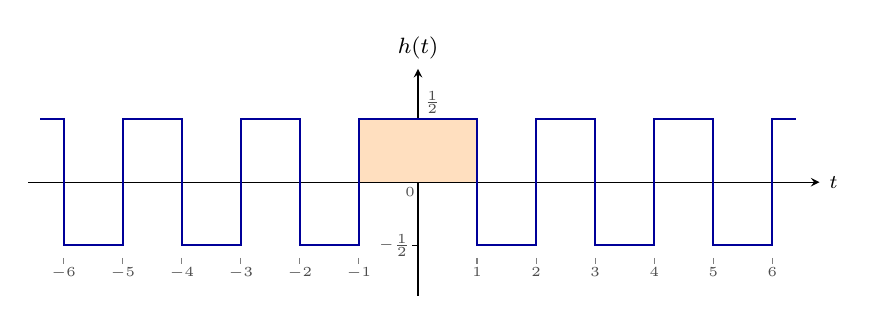
\begin{tikzpicture}[x=0.75cm,y=1.6cm]
  \taxes{-6.6}{6.8}{0.9}{-0.9}
  \fill[orange!25] (-1,0) rectangle (1,0.5);
  \draw[sig] (-6.4,0.5) -- (-6,0.5) -- (-6,-0.5) -- (-5,-0.5) -- (-5,0.5) -- (-4,0.5) -- (-4,-0.5) -- (-3,-0.5) -- (-3,0.5) -- (-2,0.5) -- (-2,-0.5) -- (-1,-0.5) -- (-1,0.5) -- (1,0.5) -- (1,-0.5) -- (2,-0.5) -- (2,0.5) -- (3,0.5) -- (3,-0.5) -- (4,-0.5) -- (4,0.5) -- (5,0.5) -- (5,-0.5) -- (6,-0.5) -- (6,0.5) -- (6.4,0.5);
  \foreach \p in {-6,...,-1,1,2,...,6}{\draw[gray] (\p,-0.6) -- (\p,-0.65) node[anchor=north,font=\tiny,gray!60!black,inner sep=1pt] {$\p$};}
  \node[anchor=south west,font=\tiny,gray!60!black,inner sep=1pt] at (0.05,0.52) {$\frac12$};
  \yt{-0.5}{-\frac12}
  \node[font=\footnotesize,anchor=south] at (0,0.9) {$h(t)$};
\end{tikzpicture}
\caption{满足 $x\ast h=y$ 的一个 $h(t)$：$|t|$ 的周期为 $2$、幅度 $\frac12$ 的方波。阴影是 $t=1$ 时的积分区间 $(-1,1)$，面积为 $1=y(1)$；区间平移到 $[0,2]$ 之外时，正负两半相互抵消。}
\end{figure}

\point{$h(t)$ 不唯一。}任取一个周期为 $2$、一个周期内积分为 $0$ 的函数 $p(t)$（例如 $\cos(\pi t)$、$\sin(3\pi t)$），都有 $x\ast p=\int_{t-2}^{t}p(\tau)\,\mathrm{d}\tau=0$。所以 $h+p$ 同样满足 $x\ast(h+p)=y$：输入 $x$「看不见」这类成分。这正对应被积函数中 $\sin\omega$ 为 $0$ 的那些点 $\omega=k\pi$。因此不同的数值算法可能给出形状差别很大的 $h(t)$，但只要与 $x$ 卷积，得到的 $y(t)$ 都接近三角波。

\end{document}
